\textit{Alvarenga p622 - Ejercicio 14}\\La figura de este ejercicio muestra un espejo plano $EE'$ y los pares de puntos $AA'$, $BB'$, $CC'$ y $DD'$. Indique cuáles pares de puntos son los que pueden estar representando un objeto pequeño y su imagen.
\begin{figure}[h!]
\centering
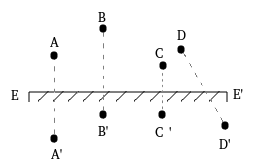
\includegraphics[width=0.5\linewidth]{enunciados/figuras/Prob14_alvarenga622.png}
 \caption{Posibles posiciones de los objetos.}
\end{figure}